
In this chapter, we put several aspects of programming together.  You will learn about the numerical methods of Riemann sums, the Trapezoidal Rule and Simpson's rule.  We'll also investigate aspects of the Traveling Salesman problem.

\section{Matlab: Numerical Methods}\label{sec:Matlab_numericalmethods}

In Calculus, you learn how to use Riemann sums, the Trapezoidal Rule and Simpson's rule to approximate definite integrals, which represent area under a curve for positive functions $f(x)$.
\[
\textrm{The area between the function and the} \, x \textrm{-axis} 
=
\int_a^b f(x) \, dx 
\]

Each involves finding the sum of areas of approximating shapes. Given a function $f(x)$ defined on an interval $[a,b]$, and a value $n$, the process is as follows.

\begin{enumerate}
\item First subdivide the interval $[a,b]$ into $n$ equal subintervals.  
\item Assign $x_0=a, x_1$ as the right endpoint of the first subinterval, $x_2$ as the right endpoint of the second subinterval, $\cdots$ , $x_n$ as the right endpoint of the $n$th interval (that is $x_n = b$).\\
\\
For example, if $a=0, b=1, n=4$, then $x_0=0, x_1=.25, x_2=.5, x_3=.75$ and $x_4=1$.\\
\\
In this example, note that even though $n=4$, there are five $x$ values.
\item Next, calculate the values $f(x_0), f(x_1), f(x_2),\cdots, f(x_n)$ by substituting the $x_i$ values into $f(x)$.
\end{enumerate}

The formulas for each of the methods are:\\
\\
\textbf{Riemann Sum:}
\[
\int_a^b f(x) \, dx
\approx
\left(\frac{b-a}{n}\right) 
\left[
f(x_0) + f(x_1) + f(x_2) + \cdots +f(x_{n-2}) + f(x_{n-1})
\right]
\]

\textbf{Trapezoidal Rule:}
\[
\int_a^b f(x) \, dx
\approx
\left(\frac{b-a}{2n}\right) 
\left[
f(x_0) + 2f(x_1) + 2f(x_2) + \cdots + 2f(x_{n-2}) + 2f(x_{n-1})+f(x_n))
\right]
\]

\textbf{Simpson's Rule:}
\[
\int_a^b f(x) \, dx
\approx
\left(\frac{b-a}{3n}\right) 
\left[
f(x_0) + 4f(x_1) + 2f(x_2) + \cdots + 2f(x_{n-2}) + 4f(x_{n-1})+f(x_n))
\right]
\]
NOTE:  The pattern of coefficients in the Trapezoidal rule is 
$1,2,2,2,\cdots, 2, 2, 1$ (each of the middle terms is a 2). In Simpson's rule, the pattern is
$1,4,2,4,2,4,\cdots,2,4,2,4,1$ where the middle terms start with a 4, alternate between 2 and 4, and end on a 4 (important!!).  This last fact forces $n$ to be an even number for Simpson's rule to work.\\

\noindent{\bf Homework}\\

Write a Matlab \textbf{function} with the following details.\\
\\
$\bullet$ Name the function appropriately (mine could be siemerstj\underline{ }num\underline{ }methods)\\
$\bullet$ Comment the function appropriately including a description of the usage.\\
$\bullet$ The function should have three inputs ${\bf a, b, n}$ \\
$\bullet$ The function should have three outputs \textbf{Rsum, Tsum, Ssum}\\
$\bullet$ Once the function is run, a \textbf{menu} should appear with three choices of functions to choose from:
\[
x^2, \quad \sin x, \quad \sqrt{\frac{1}{2\pi}} e^{-x^2/2}
\]
$\bullet$ Once the user clicks on a function from the menu, the function should compute the three approximations and output the values in a nice format (Hint: use \cour{fprintf}).\\
$\bullet$ If $n$ is not even, then only the Rsum and Tsum should be displayed with a message saying the Ssum could not be calculated.\\
\\
Here is a sample run.  Suppose I typed this :\\
\\
\cour{>> [Rsum,Tsum,Ssum]=siemerstj\underline{ }num\underline{ }methods(0,1,6)}\\
\\
and then clicked on the $x^2$ button in the menu. Then the output should be:\\
\\
\cour{Rsum=.25463, Tsum=.3380, Ssum=0.33333}

\section{Matlab Traveling Salesman}\label{sec:Matlab_travelingsalesman}

A famous problem in mathematics is the Traveling Salesman Problem where the minimum distance of traveling from a home city, through n cities and back to the home city.  In this program, you will simulate part of this problem.\\
\\
{\bf Homework}\\

You will write a Matlab \cour{function} with the following details:\\
\\
$\bullet$  Name the function appropriately (like siemerstjTravelingSalesman)\\
$\bullet$  Comment the function appropriately including a description of the usage.\\
$\bullet$  The function has \textbf{one input} (a matrix of locations of the cities) and \textbf{no outputs}.\\
$\bullet$  Once the function is run, a figure will appear with the cities indicated with one type of symbol and the home city (at the {\bf origin}) with another.\\
$\bullet$  The user will select cities one at a time with the mouse.\\
$\bullet$  Each time a city is selected, a line is drawn from the previous city with a message of the city selected.\\
$\bullet$  Repeat until all cities are selected.\\
$\bullet$  Once the last remaining city is selected, a line is drawn back to the home city and the total distance of the trip is displayed.\\

Code execution:\\

Suppose I enter \cour{siemerstjTravelingSalesman([1 1;2 2;3 10])}.  Then the following picture chould appear.  The ``home base'' plotted as a green asterisk at the origin and the three cities are plotted at the coordinates $(1,1), (2,2), (3,10)$.  Note that the screen is a little larger so that the cities do not fall on the edge of the plot (see either \cour{xlim$\backslash$ylim} or \cour{axes}).\\
\\
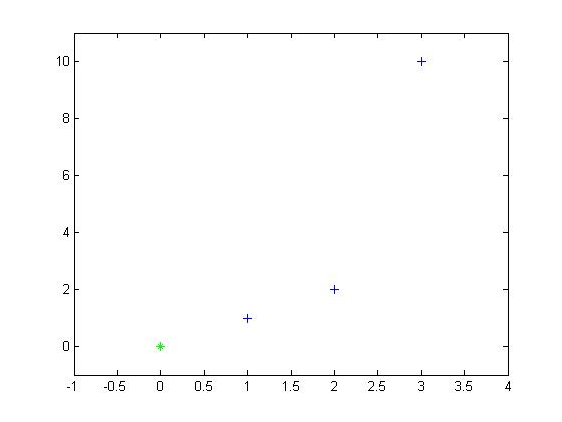
\includegraphics[scale=0.5]{figures/matlab_ts1.png}\\
\\
When I click on the closest city (at $(1,1)$), I now have\\
\\
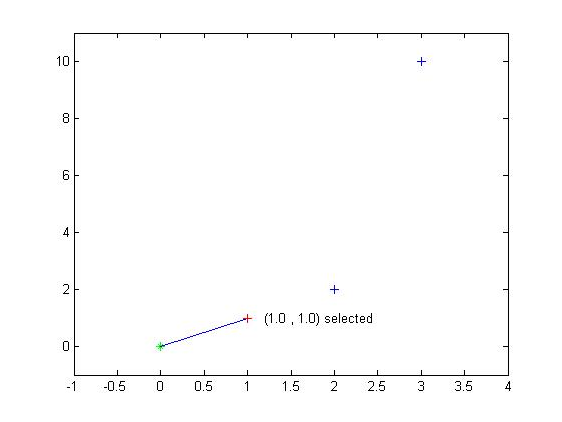
\includegraphics[scale=0.5]{figures/matlab_ts2.png}\\
\\
Click the next city...\\
\\
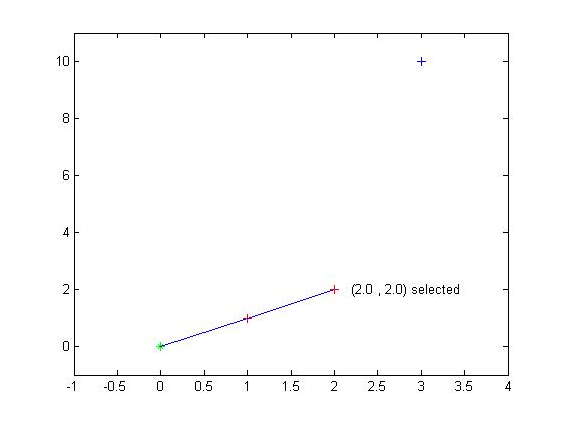
\includegraphics[scale=0.5]{figures/matlab_ts3.png}\\
\\
Finish with the last city...\\
\\
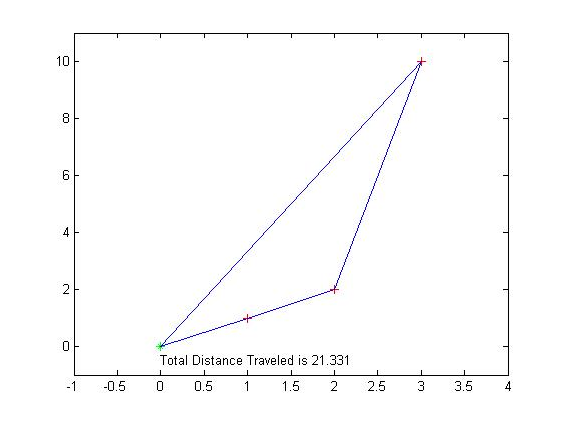
\includegraphics[scale=0.5]{figures/matlab_ts4.png}\\

A few issues arise as you work through the code for this project:\\
\\
1) Does the user have to click exactly on top of a city, or can you write the code so that they can click close to the city (and how ``close'' is close enough?).\\
2) How do you keep the user from selecting the same city twice?\\
3) How do you make the text for one city ``disappear'' when the next city is clicked? (see \cour{set} command for one possibility).\\


%\definition{def:lineintegral}{\textbf{TITLE}}
%
%\keyidea{idea:lineintprops}{\textbf{TITLE}}
%
%\printexercises{exercises/mathcad_introduction_exercises}
